\chapter{Reprodução sexuada das plantas com flores}\label{ch:b2:angiosperm-reproduction}

Um pomar de macieiras em maio está branco de \omterm{def:b2:angiosperm-reproduction:flower}{flores} e barulhento de
abelhas; em outubro, as mesmas árvores estão carregadas de \omterm{def:b2:angiosperm-reproduction:seed}{frutos}, cada
maçã com dez \omterm{def:b2:angiosperm-reproduction:seed}{sementes}, cada \omterm{def:b2:angiosperm-reproduction:seed}{semente} uma árvore embrionária envolta
numa reserva de alimento. Toda essa transformação --- a \omterm{def:b2:angiosperm-reproduction:flower}{flor}, o \omterm{def:b2:plant-life-cycles:heterospory}{pólen}
levado por um inseto, o tubo que cresce através do estilete, a \omterm{prop:b2:angiosperm-reproduction:double}{dupla
fecundação} que produz ao mesmo tempo um embrião e seu suprimento de
alimento, o \omterm{def:b2:angiosperm-reproduction:flower}{ovário} que incha num \omterm{def:b2:angiosperm-reproduction:seed}{fruto} feito para ser comido --- é a
invenção que fez das plantas com \omterm{def:b2:angiosperm-reproduction:flower}{flores}, em cem milhões de anos, as
plantas dominantes em terra firme. Este capítulo a acompanha da \omterm{def:b2:angiosperm-reproduction:flower}{flor} à
\omterm{def:b2:angiosperm-reproduction:seed}{semente} dispersada.

\section{A flor}

\begin{definition}[As partes de uma flor]\label{def:b2:angiosperm-reproduction:flower}
\index{flor}\index{estame}\index{carpelo}\index{ovário}\index{estigma}
Uma \emph{flor} é um ramo curto cujas folhas se transformaram em
quatro verticilos. Por fora, as \emph{sépalas} (juntas, o cálice)
protegem o botão; depois vêm as \emph{pétalas} (a corola), que
anunciam; depois os \emph{estames}, cada um um filete que leva uma
\emph{antera} com quatro sacos polínicos; e, no centro, um ou mais
\emph{carpelos}, cada um dobrado e fechado num \emph{pistilo} com um
\emph{estigma} receptivo, um \emph{estilete} e um \emph{ovário} que
encerra os \emph{\omterm{def:b2:plant-life-cycles:heterospory}{óvulos}}. Uma flor com estames e carpelos é
\emph{hermafrodita} (a maioria das espécies); as plantas
\emph{monoicas} têm flores masculinas e femininas separadas num mesmo
indivíduo (milho, carvalho, aveleira), e as espécies \emph{dioicas}, em
indivíduos separados (azevinho, salgueiro, tamareira). Todo o sentido
do carpelo fechado --- o caráter que dá nome às angiospermas --- é que
os \omterm{def:b2:plant-life-cycles:heterospory}{óvulos} ficam encerrados: o \omterm{def:b2:plant-life-cycles:heterospory}{pólen} nunca os alcança diretamente, mas
precisa crescer até eles através dos tecidos da planta, o que permite
à planta escolher.
\end{definition}

\begin{omfigure}
\begin{tikzpicture}[every node/.style={font=\scriptsize}]
  % receptacle and pedicel
  \draw[thick] (0,-2.6) -- (0,-1.6);
  \draw[thick, fill=omExo!20] (-0.9,-1.6) .. controls (-1.0,-1.0) and (1.0,-1.0) .. (0.9,-1.6) -- cycle;
  % sepals
  \foreach \s in {-1,1} \draw[thick, fill=omExo!45] (0.6*\s,-1.4) .. controls (2.0*\s,-1.2) and (2.6*\s,-0.2) .. (2.8*\s,0.6) .. controls (2.0*\s,0.2) and (1.2*\s,-0.6) .. (0.6*\s,-1.4);
  % petals
  \foreach \s in {-1,1} \draw[thick, fill=omThm!15] (0.5*\s,-1.2) .. controls (1.6*\s,0.4) and (2.2*\s,1.8) .. (1.6*\s,3.0) .. controls (1.0*\s,2.0) and (0.5*\s,0.8) .. (0.5*\s,-1.2);
  % ovary with ovules
  \draw[thick, fill=omDef!12] (0,-0.7) ellipse (0.55 and 0.75);
  \foreach \p in {(-0.22,-0.5),(-0.22,-0.9),(0.22,-0.5),(0.22,-0.9)} \draw[thick, omDef, fill=omDef!40] \p circle (0.11);
  % style and stigma
  \draw[thick, fill=omDef!12] (-0.1,0.05) rectangle (0.1,1.9);
  \draw[thick, fill=omDef!40] (0,2.0) ellipse (0.28 and 0.14);
  % stamens
  \foreach \s in {-1,1} { \draw[thick] (0.35*\s,-1.0) .. controls (0.6*\s,0.2) .. (0.9*\s,1.5); \draw[thick, fill=omProp!60] (0.9*\s,1.6) ellipse (0.14 and 0.32); }
  % labels: right side
  \draw (0.28,2.0) -- (3.2,2.6) node[right] {estigma};
  \draw (0.1,1.2) -- (3.2,1.9) node[right] {estilete};
  \draw (0.55,-0.6) -- (3.2,1.2) node[right] {ovário};
  \draw (0.22,-0.9) -- (3.2,0.5) node[right] {óvulo};
  \draw (2.6,0.35) -- (3.2,-0.4) node[right] {sépala};
  % labels: left side
  \draw (-1.5,2.4) -- (-2.6,2.8) node[left] {pétala};
  \draw (-0.95,1.9) -- (-2.6,1.9) node[left] {antera};
  \draw (-0.65,0.6) -- (-2.6,0.9) node[left] {filete};
  \draw (0,-2.2) -- (-2.6,-2.2) node[left] {receptáculo e pedúnculo};
  \node[anchor=west, align=left] at (5.4,0.5) {estigma + estilete + ovário\\$=$ o carpelo (pistilo)};
  \node[anchor=west, align=left] at (5.4,-0.8) {antera + filete\\$=$ o estame};
\end{tikzpicture}

{\small Uma \omterm{def:b2:angiosperm-reproduction:flower}{flor} em corte longitudinal: sépalas, pétalas, \omterm{def:b2:angiosperm-reproduction:flower}{estames}
(filete e antera) e, no centro, o \omterm{def:b2:angiosperm-reproduction:flower}{carpelo} --- \omterm{def:b2:angiosperm-reproduction:flower}{estigma}, estilete e
\omterm{def:b2:angiosperm-reproduction:flower}{ovário} ---, que encerra os \omterm{def:b2:plant-life-cycles:heterospory}{óvulos}.}
\end{omfigure}

\begin{omfigure}
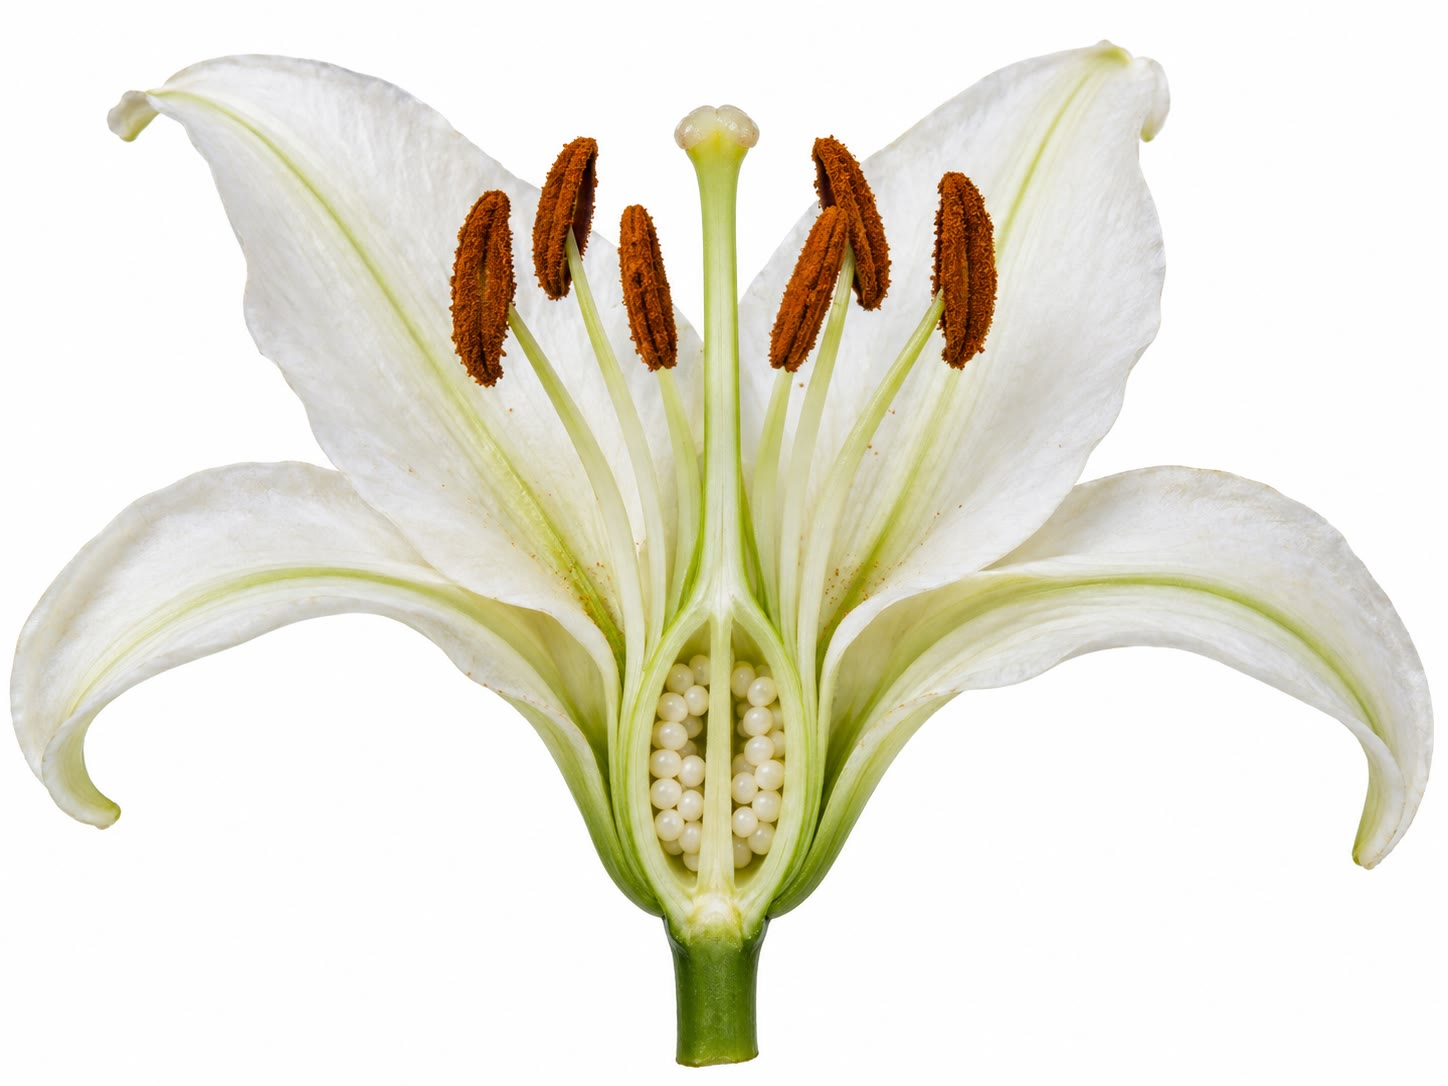
\includegraphics[width=0.55\linewidth]{images/book4/ai/b4-06-lily-dissected.jpg}

{\small Um lírio cortado ao comprido: seis \omterm{def:b2:angiosperm-reproduction:flower}{estames} com anteras
carregadas de \omterm{def:b2:plant-life-cycles:heterospory}{pólen}, o longo estilete com seu \omterm{def:b2:angiosperm-reproduction:flower}{estigma} pegajoso e o
\omterm{def:b2:angiosperm-reproduction:flower}{ovário} aberto para mostrar as fileiras de \omterm{def:b2:plant-life-cycles:heterospory}{óvulos}.}
\end{omfigure}

\section{Os dois gametófitos}

\begin{proposition}[O pólen: o gametófito masculino]\label{prop:b2:angiosperm-reproduction:pollen}
\index{grão de pólen}\index{microsporogênese}\index{esporopolenina}
Em cada saco polínico, células-mães \omterm{def:b2:meiosis-heredity:meiosis}{diploides} sofrem \omterm{def:b2:meiosis-heredity:meiosis}{meiose} e dão
tétrades de \emph{\omterm{def:b2:plant-life-cycles:heterospory}{micrósporos}}. Cada \omterm{def:b2:plant-life-cycles:heterospory}{micrósporo} se divide uma vez, de
modo desigual, numa grande \emph{célula vegetativa} e numa pequena
\emph{célula generativa} contida nela; a célula generativa se divide
mais uma vez, antes ou depois da \omterm{def:b2:angiosperm-reproduction:pollination}{polinização}, em duas \emph{células
espermáticas}. O \emph{\omterm{prop:b2:angiosperm-reproduction:pollen}{grão de pólen}} maduro é, assim, um organismo
\omterm{def:b2:meiosis-heredity:meiosis}{haploide} de três células --- o \omterm{def:b2:plant-life-cycles:cycles}{gametófito} masculino inteiro --- de
\qtyrange{10}{100}{\micro m}, selado numa parede cuja camada externa de
\emph{esporopolenina}, o polímero biológico mais resistente que se
conhece, é esculpida com espinhos, poros e sulcos característicos da
espécie, e é por isso que o \omterm{def:b2:plant-life-cycles:heterospory}{pólen} identifica plantas em sedimentos com
dezenas de milhões de anos. O grão é liberado desidratado e sobrevive
de horas (gramíneas) a semanas (algumas árvores), até alcançar um
\omterm{def:b2:angiosperm-reproduction:flower}{estigma}.
\end{proposition}

\begin{omfigure}
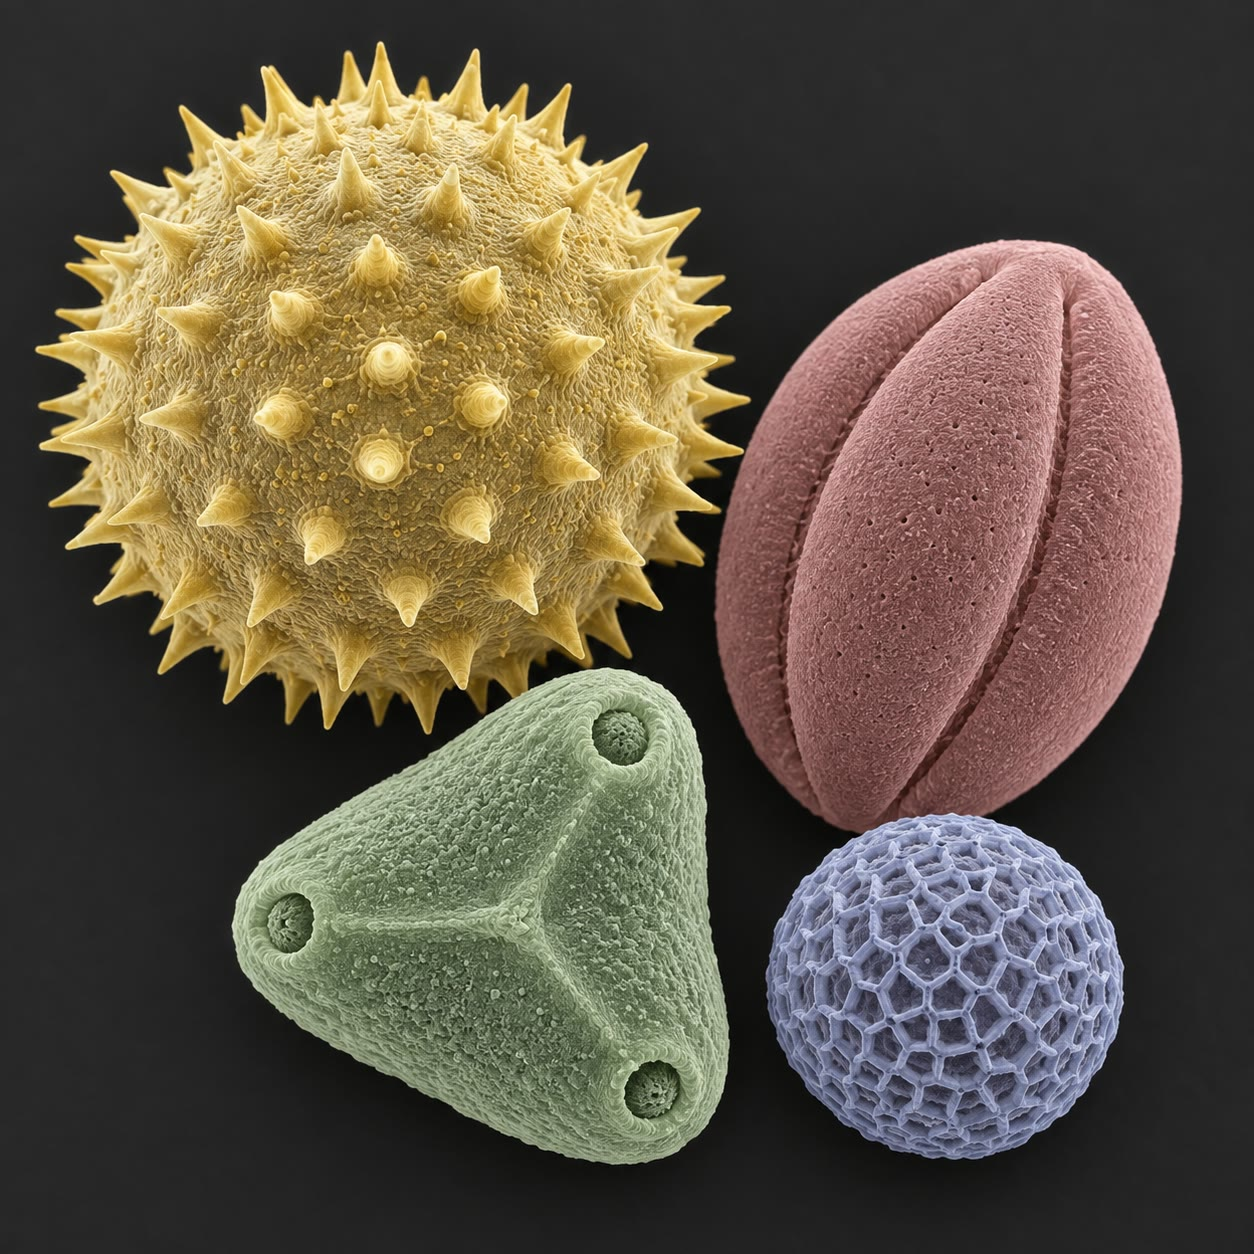
\includegraphics[width=0.45\linewidth]{images/book4/ai/b4-06-pollen-sem.jpg}

{\small \omterm{prop:b2:angiosperm-reproduction:pollen}{Grãos de pólen} ao microscópio eletrônico de varredura: a parede
de esporopolenina de cada espécie tem sua própria escultura ---
espinhos, sulcos, poros, uma rede ---, pela qual pode ser reconhecida.}
\end{omfigure}

\begin{proposition}[O saco embrionário: o gametófito feminino]\label{prop:b2:angiosperm-reproduction:embryosac}
\index{saco embrionário}\index{megasporogênese}\index{núcleos polares}
Em cada \omterm{def:b2:plant-life-cycles:heterospory}{óvulo}, uma célula \omterm{def:b2:meiosis-heredity:meiosis}{diploide} do nucelo sofre \omterm{def:b2:meiosis-heredity:meiosis}{meiose}; três dos
quatro \omterm{def:b2:plant-life-cycles:heterospory}{megásporos} degeneram, e o quarto cresce, por três mitoses sem
divisão celular, num \emph{\omterm{prop:b2:angiosperm-reproduction:embryosac}{saco embrionário}} de oito núcleos e sete
células: na extremidade micropilar, a \emph{oosfera}, ladeada por duas
\emph{sinérgides}; na extremidade oposta, três células
\emph{antípodas}; no meio, uma grande \emph{célula central} que contém
dois \emph{\omterm{prop:b2:angiosperm-reproduction:embryosac}{núcleos polares}}. Esse saco, envolto pelo nucelo e por dois
tegumentos com uma micrópila, é o \omterm{def:b2:plant-life-cycles:cycles}{gametófito} feminino inteiro --- sete
células, onde um \omterm{def:b2:plant-life-cycles:moss}{musgo} tinha uma planta. Os dois \omterm{prop:b2:angiosperm-reproduction:embryosac}{núcleos polares} são
geneticamente idênticos à oosfera, fato que importa para o endosperma.
\end{proposition}

\begin{omfigure}
\begin{tikzpicture}[every node/.style={font=\scriptsize}]
  % pollen grain
  \begin{scope}
    \draw[very thick, omProp!80!black, fill=omProp!15] (0,0) circle (1.1);
    \draw[thick, omProp!80!black] (0,0) circle (0.95);
    \foreach \a in {0,30,...,330} \draw[omProp!80!black, thick] (\a:1.1) -- (\a:1.25);
    \draw[thick, fill=omDef!25] (0.15,-0.2) ellipse (0.55 and 0.4); \node[font=\tiny] at (0.15,-0.2) {vegetativa};
    \draw[thick, fill=omThm!30] (-0.3,0.45) ellipse (0.22 and 0.14); \draw[thick, fill=omThm!30] (0.2,0.5) ellipse (0.22 and 0.14);
    \draw[omThm] (0.0,0.62) -- (0.0,1.5); \node[omThm, anchor=south] at (0.0,1.5) {duas células espermáticas};
    \node[below, align=center] at (0,-1.4) {grão de pólen ($n$)\\3 células, parede de esporopolenina};
  \end{scope}
  % ovule with embryo sac
  \begin{scope}[xshift=5.5cm]
    \draw[thick, fill=omExo!25] (0,0) ellipse (1.5 and 2.1);
    \draw[thick, fill=omExo!10] (0,0) ellipse (1.15 and 1.75);
    \fill[white] (-0.3,1.7) rectangle (0.3,2.2); \draw[thick] (-0.3,1.7) -- (-0.3,2.15); \draw[thick] (0.3,1.7) -- (0.3,2.15);
    \draw[thick, fill=white] (0,0) ellipse (0.7 and 1.35);
    % cells: egg + synergids top, central, antipodals bottom
    \draw[thick, fill=omThm!30] (0,0.95) circle (0.17); \node[omThm, anchor=west] at (1.6,1.2) {oosfera};
    \draw[thick, fill=omDef!25] (-0.35,1.0) circle (0.14); \draw[thick, fill=omDef!25] (0.35,1.0) circle (0.14); \node[anchor=west] at (1.6,0.75) {duas sinérgides};
    \draw[thick, fill=omDef!10] (0,0) ellipse (0.55 and 0.6); \fill[omDef!80!black] (-0.15,0.05) circle (0.09); \fill[omDef!80!black] (0.15,0.05) circle (0.09);
    \node[anchor=west, align=left] at (1.6,0.1) {célula central com\\dois núcleos polares};
    \foreach \x in {-0.3,0,0.3} \draw[thick, fill=omDef!25] (\x,-1.0) circle (0.13); \node[anchor=west] at (1.6,-1.0) {três antípodas};
    \draw (0.35,2.0) -- (1.6,2.0) node[right] {micrópila};
    \draw (1.3,-0.9) -- (1.6,-1.6) node[right] {tegumentos};
    \draw (0.9,-1.35) -- (1.6,-2.1) node[right] {nucelo};
    \draw (1.6,1.2) -- (0.17,0.95); \draw (1.6,0.75) -- (0.49,1.0); \draw (1.6,0.1) -- (0.55,0.05); \draw (1.6,-1.0) -- (0.43,-1.0);
    \node[below, align=center] at (0,-2.3) {óvulo com saco embrionário ($n$)\\7 células, 8 núcleos};
  \end{scope}
\end{tikzpicture}

{\small Os dois \omterm{def:b2:plant-life-cycles:cycles}{gametófitos} de uma planta com \omterm{def:b2:angiosperm-reproduction:flower}{flores}, ambos reduzidos a
poucas células: o \omterm{prop:b2:angiosperm-reproduction:pollen}{grão de pólen} de três células e o \omterm{prop:b2:angiosperm-reproduction:embryosac}{saco embrionário}
de sete células dentro do \omterm{def:b2:plant-life-cycles:heterospory}{óvulo}.}
\end{omfigure}

\section{A polinização}

\begin{definition}[A polinização e seus agentes]\label{def:b2:angiosperm-reproduction:pollination}
\index{polinização}\index{síndrome de polinização}\index{néctar}
A \emph{polinização} é a transferência do \omterm{def:b2:plant-life-cycles:heterospory}{pólen} de uma antera para um
\omterm{def:b2:angiosperm-reproduction:flower}{estigma}; \emph{autopolinização} numa mesma \omterm{def:b2:angiosperm-reproduction:flower}{flor} ou planta,
\emph{polinização cruzada} entre plantas. As \omterm{def:b2:angiosperm-reproduction:flower}{flores} \emph{polinizadas
pelo vento} (gramíneas, carvalhos, bétulas, tanchagens) são pequenas,
verdes, sem perfume, com grandes \omterm{def:b2:angiosperm-reproduction:flower}{estigmas} plumosos e quantidades
enormes de \omterm{def:b2:plant-life-cycles:heterospory}{pólen} liso e seco; sua razão \omterm{def:b2:plant-life-cycles:heterospory}{pólen}/\omterm{def:b2:plant-life-cycles:heterospory}{óvulo} chega a um milhão.
As \omterm{def:b2:angiosperm-reproduction:flower}{flores} \emph{polinizadas por animais} pagam seu transportador:
\emph{néctar} (solução açucarada secretada por nectários), o próprio
\omterm{def:b2:plant-life-cycles:heterospory}{pólen}, óleos, perfume; e anunciam com cor, forma e odor ajustados aos
sentidos do transportador --- guias de néctar ultravioleta para as
abelhas, que veem o ultravioleta e não o vermelho; \omterm{def:b2:angiosperm-reproduction:flower}{flores} tubulares
vermelhas e sem perfume para os \omterm{def:b2:angiosperm-reproduction:flower}{beija-flores}; \omterm{def:b2:angiosperm-reproduction:flower}{flores} brancas, muito
perfumadas, de abertura noturna e tubos profundos para as mariposas;
\omterm{def:b2:angiosperm-reproduction:flower}{flores} castanhas e fétidas para as moscas-varejeiras; \omterm{def:b2:angiosperm-reproduction:flower}{flores}
robustas, pálidas e noturnas para os morcegos. Cada conjunto desses
traços é uma \emph{síndrome de polinização}, e o ajuste entre \omterm{def:b2:angiosperm-reproduction:flower}{flor} e
polinizador é o caso clássico de \emph{coevolução}: Darwin previu, a
partir do esporão nectarífero de \qty{30}{cm} de uma orquídea de
Madagascar, uma mariposa com uma probóscide de \qty{30}{cm},
encontrada quarenta anos depois.
\end{definition}

\begin{omfigure}
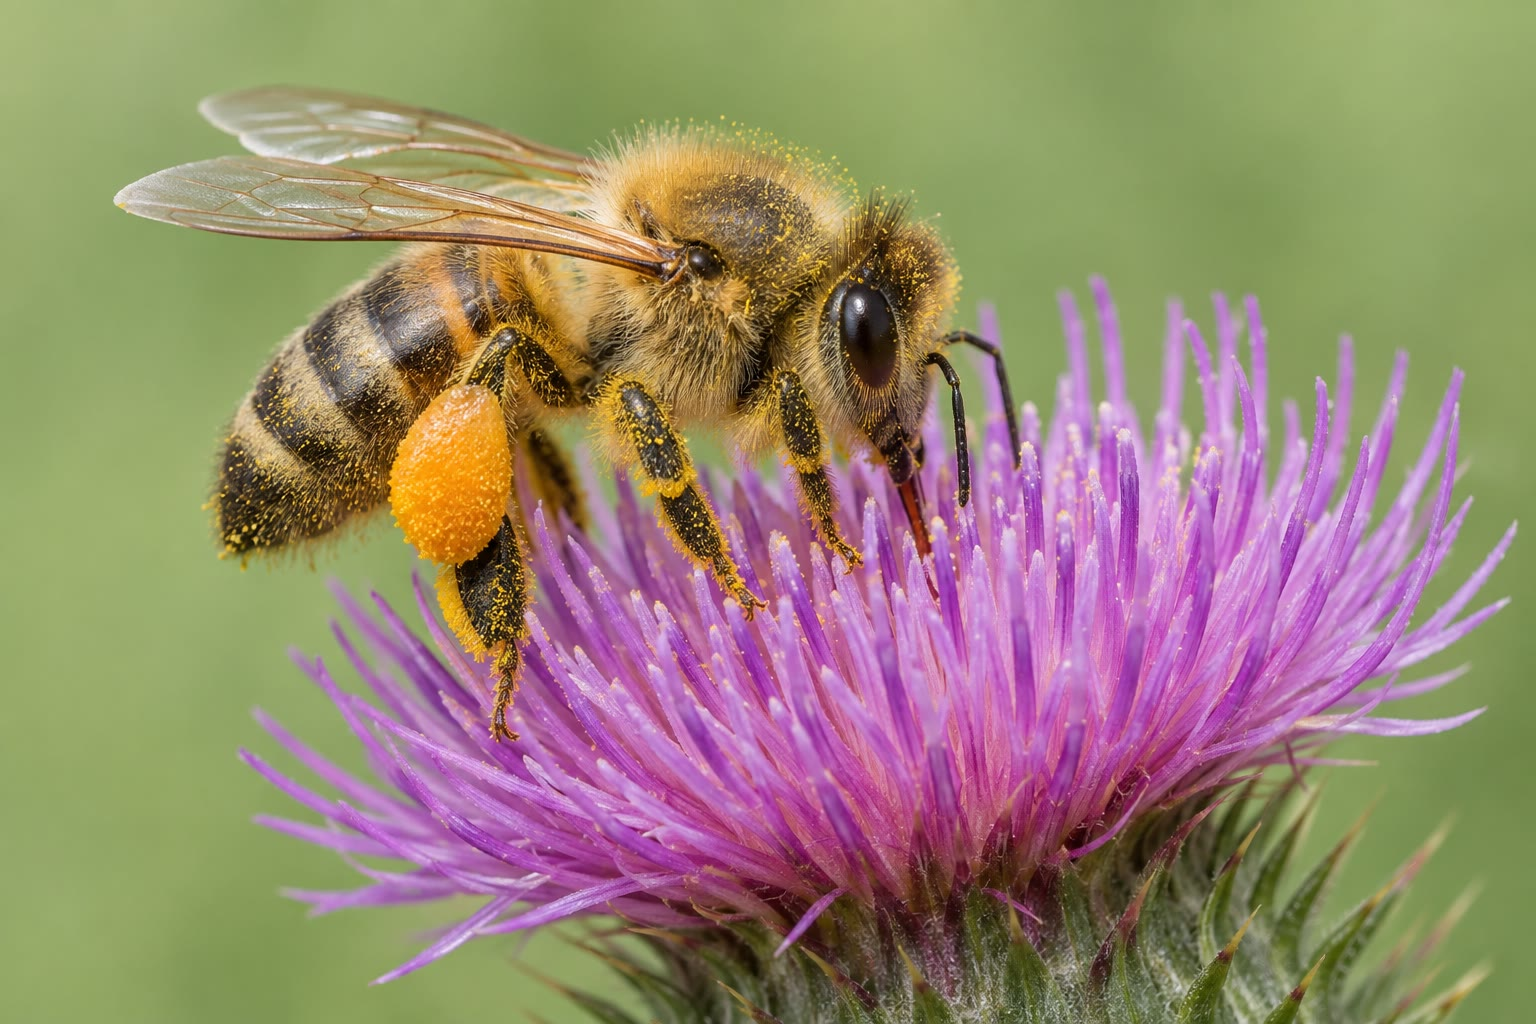
\includegraphics[width=0.58\linewidth]{images/book4/ai/b4-06-bee-on-flower.jpg}

{\small Uma abelha-europeia num cardo: o \omterm{def:b2:plant-life-cycles:heterospory}{pólen} cobre seu corpo e enche
as corbículas das patas traseiras; parte dele alcançará o \omterm{def:b2:angiosperm-reproduction:flower}{estigma} do
próximo cardo que ela visitar. A cor púrpura, uma plataforma de pouso
e \omterm{def:b2:angiosperm-reproduction:pollination}{néctar} abundante formam a síndrome da abelha.}
\end{omfigure}

\begin{proposition}[Evitar a autofecundação]\label{prop:b2:angiosperm-reproduction:selfing}
\index{autoincompatibilidade}\index{heterostilia}\index{dicogamia}
Uma \omterm{def:b2:angiosperm-reproduction:flower}{flor} hermafrodita poderia fecundar a si mesma, e muitas o fazem
(ervilha, trigo, tomate); mas a autofecundação expõe \omterm{def:b2:meiosis-heredity:vocabulary}{alelos} \omterm{def:b2:meiosis-heredity:vocabulary}{recessivos}
deletérios (\emph{depressão por endogamia}), e a maioria das espécies a
impede. No tempo: a \emph{dicogamia}, com anteras e \omterm{def:b2:angiosperm-reproduction:flower}{estigma} amadurecendo
em momentos diferentes (protandria na maioria das umbelíferas e das
compostas). No espaço: a \emph{hercogamia}, com anteras e \omterm{def:b2:angiosperm-reproduction:flower}{estigma}
mantidos separados, como na \emph{heterostilia} das prímulas, cujas
\omterm{def:b2:angiosperm-reproduction:flower}{flores} longistilas (estilete longo, anteras baixas) e brevistilas
(estilete curto, anteras altas) depositam o \omterm{def:b2:plant-life-cycles:heterospory}{pólen} em partes diferentes
do corpo de um inseto. Bioquimicamente: a \emph{autoincompatibilidade},
um sistema de reconhecimento em que o \omterm{def:b2:plant-life-cycles:heterospory}{pólen} que leva um \omterm{def:b2:meiosis-heredity:vocabulary}{alelo} $S$
compartilhado com o pistilo é rejeitado. Na incompatibilidade
\emph{gametofítica} (macieira, cerejeira, petúnia, gramíneas), é o
próprio \omterm{def:b2:meiosis-heredity:vocabulary}{alelo} $S$ \omterm{def:b2:meiosis-heredity:meiosis}{haploide} do \omterm{def:b2:plant-life-cycles:heterospory}{pólen} que decide: um pistilo
$S_1S_2$ detém os tubos $S_1$ e $S_2$ no estilete, de modo que o \omterm{def:b2:plant-life-cycles:heterospory}{pólen}
de uma planta $S_1S_3$ é compatível pela metade e o de uma $S_3S_4$,
por inteiro. Na incompatibilidade \emph{esporofítica} (couve,
girassol), é o \omterm{def:b2:meiosis-heredity:vocabulary}{genótipo} \omterm{def:b2:meiosis-heredity:meiosis}{diploide} da planta que produziu o \omterm{def:b2:plant-life-cycles:heterospory}{pólen} que
decide, na superfície do \omterm{def:b2:angiosperm-reproduction:flower}{estigma}. Um \omterm{def:b2:meiosis-heredity:vocabulary}{alelo} $S$ raro é compatível com
quase todos os parceiros, de modo que a seleção mantém dezenas de
\omterm{def:b2:meiosis-heredity:vocabulary}{alelos} numa população.
\end{proposition}
\begin{proof}[Evidências]
Darwin (1862, 1877) cruzou prímulas à mão: o \omterm{def:b2:plant-life-cycles:heterospory}{pólen} de uma \omterm{def:b2:angiosperm-reproduction:flower}{flor}
brevistila sobre um \omterm{def:b2:angiosperm-reproduction:flower}{estigma} longistilo (uma união ``legítima'') formava
cápsulas cheias; longistila sobre longistila ou brevistila sobre
brevistila (``ilegítimas'') formavam poucas \omterm{def:b2:angiosperm-reproduction:seed}{sementes} ou nenhuma,
embora as plantas fossem sadias e o \omterm{def:b2:plant-life-cycles:heterospory}{pólen} estivesse vivo. Ele concluiu
que as duas formas estavam mutuamente adaptadas ao cruzamento e
protegidas da autofecundação e, contando as \omterm{def:b2:angiosperm-reproduction:seed}{sementes} por cápsula em
milhares de cruzamentos, mediu o custo da autofecundação em dezenas de
espécies: os descendentes autofecundados eram mais baixos, mais leves
e menos férteis, geração após geração.
\end{proof}

\begin{omfigure}
\begin{tikzpicture}[every node/.style={font=\scriptsize}]
  % pistil S1S2 with pollen tubes
  \draw[thick, fill=omDef!10] (-0.5,0) rectangle (0.5,3.2);
  \draw[thick, fill=omDef!30] (0,3.3) ellipse (0.7 and 0.2);
  \draw[thick, fill=omDef!12] (0,-0.6) ellipse (0.9 and 0.7);
  \node at (0,-0.6) {ovário};
  \node[anchor=east] at (-1.1,3.3) {estigma de uma planta $S_1S_2$};
  % pollen grains
  \draw[thick, fill=omThm!40] (-0.35,3.75) circle (0.13); \node[omThm, left] at (-0.5,3.75) {$S_1$};
  \draw[thick, fill=omThm!40] (0,3.75) circle (0.13); \node[omThm, anchor=south] at (0,3.92) {$S_2$};
  \draw[thick, fill=omExo!70!black] (0.35,3.75) circle (0.13); \node[right] at (0.5,3.75) {$S_3$};
  % tubes: S1 and S2 stop in the style, S3 reaches the ovary
  \draw[thick, omThm] (-0.35,3.3) -- (-0.35,2.3); \node[omThm, left, align=right] at (-0.55,2.3) {tubo $S_1$\\detido};
  \draw[thick, omThm] (0,3.3) -- (0,2.0);
  \draw[thick, omExo!70!black] (0.35,3.3) -- (0.35,-0.2) -- (0.2,-0.5);
  \node[right, align=left] at (0.55,0.9) {tubo $S_3$\\alcança um óvulo};
  \node[anchor=west, align=left, text width=6cm] at (3.2,3.2) {autoincompatibilidade gametofítica: um tubo polínico cujo próprio alelo $S$ coincide com um dos alelos do pistilo é detido no estilete};
  \node[anchor=west, align=left, text width=6cm] at (3.2,1.4) {pólen de uma planta $S_1S_2$: 0 compatível\\de $S_1S_3$: metade\\de $S_3S_4$: todo};
\end{tikzpicture}

{\small A autoincompatibilidade gametofítica. Num pistilo $S_1S_2$, os
tubos que levam $S_1$ ou $S_2$ são detidos no estilete; um tubo $S_3$
cresce até o \omterm{def:b2:angiosperm-reproduction:flower}{ovário}.}
\end{omfigure}

\section{A fecundação}

\begin{theorem}[O tubo polínico]\label{thm:b2:angiosperm-reproduction:tube}
\index{tubo polínico}
Um \omterm{prop:b2:angiosperm-reproduction:pollen}{grão de pólen} sobre um \omterm{def:b2:angiosperm-reproduction:flower}{estigma} compatível se reidrata e forma um
\emph{\omterm{thm:b2:angiosperm-reproduction:tube}{tubo polínico}}: a célula vegetativa se alonga por crescimento
apical, depositando parede nova no ápice a uma taxa de
\qtyrange{0.1}{1}{cm/h}, digerindo seu caminho através do tecido
transmissor do estilete e alimentando-se dele. O tubo leva as duas
células espermáticas em sua ponta; é guiado no último trecho por
peptídeos secretados pelas sinérgides, entra no \omterm{def:b2:plant-life-cycles:heterospory}{óvulo} pela micrópila,
rompe-se dentro de uma sinérgide e libera as células espermáticas. Um
tubo que atravessa um estilete de comprimento $L$ à velocidade $v$
leva $L/v$: algumas horas numa cerejeira, um dia inteiro no milho,
cujos ``cabelos'' são estiletes de \qty{20}{cm}. A viabilidade do \omterm{def:b2:plant-life-cycles:heterospory}{pólen}
impõe um relógio: o \omterm{def:b2:plant-life-cycles:heterospory}{pólen} das gramíneas morre em horas, de modo que um
\omterm{def:b2:angiosperm-reproduction:flower}{estigma} precisa ser alcançado depressa.
\end{theorem}
\begin{proof}
O tempo é o comprimento dividido pela taxa de crescimento; no milho,
\qty{20}{cm} a \qty{1}{cm/h} dão \qty{20}{h}. O próprio tubo consiste
quase inteiramente de parede e de uma fina película de citoplasma
atrás da ponta, de modo que as reservas da célula vegetativa, somadas
ao que ela absorve do estilete, bastam para um comprimento mil vezes
maior que o diâmetro do grão.
\end{proof}

\begin{proposition}[A dupla fecundação]\label{prop:b2:angiosperm-reproduction:double}
\index{dupla fecundação}\index{endosperma}
Das duas células espermáticas entregues pelo tubo, uma se funde com a
oosfera e forma o \emph{zigoto} \omterm{def:b2:meiosis-heredity:meiosis}{diploide}, a partir do qual cresce o
embrião; a outra se funde com a célula central e seus dois \omterm{prop:b2:angiosperm-reproduction:embryosac}{núcleos
polares} e forma um núcleo \emph{triploide} ($3n$: dois genomas maternos,
um paterno), a partir do qual cresce o \emph{endosperma} --- um tecido
nutritivo que enche a \omterm{def:b2:angiosperm-reproduction:seed}{semente} de amido, óleo e proteína. As duas
fecundações ocorrem com minutos de diferença; na maioria das espécies,
nenhuma é bem-sucedida sem a outra, de modo que a planta só abastece as
\omterm{def:b2:angiosperm-reproduction:seed}{sementes} que levam um embrião. O endosperma é o tecido que alimenta a
humanidade: a farinha do trigo e do arroz, o fubá do milho, a polpa
branca do coco são endosperma triploide. Nas gimnospermas, a reserva
de alimento da \omterm{def:b2:angiosperm-reproduction:seed}{semente} é o \omterm{def:b2:plant-life-cycles:cycles}{gametófito} feminino, construído antes da
fecundação, venha ou não um embrião; o endosperma das angiospermas é
feito sob encomenda.
\end{proposition}
\begin{proof}[Evidências]
Nawaschin (1898), seguindo ao microscópio o \omterm{thm:b2:angiosperm-reproduction:tube}{tubo polínico} de um lírio
e de uma fritilária até o \omterm{prop:b2:angiosperm-reproduction:embryosac}{saco embrionário}, viu os dois núcleos
espermáticos deixarem o tubo, um entrando na oosfera e o outro se
fundindo com os \omterm{prop:b2:angiosperm-reproduction:embryosac}{núcleos polares}; Guignard o confirmou no ano seguinte
em outras espécies. A triploidia do endosperma decorreu das contagens
de cromossomos, e suas consequências genéticas --- o endosperma de um
grão exibindo os caracteres do genitor que forneceu o \omterm{def:b2:plant-life-cycles:heterospory}{pólen}
(\emph{xênia}), na proporção de duas doses maternas para uma paterna
--- já tinham sido notadas muito antes pelos melhoristas de milho.
\end{proof}

\begin{omfigure}
\begin{tikzpicture}[every node/.style={font=\scriptsize}, >=stealth]
  \node[draw, rounded corners, fill=omProp!15, align=center] (sp) at (0,2) {célula espermática 1 ($n$)};
  \node[draw, rounded corners, fill=omProp!15, align=center] (sp2) at (0,0) {célula espermática 2 ($n$)};
  \node[draw, rounded corners, fill=omThm!15, align=center] (egg) at (4,2) {oosfera ($n$)};
  \node[draw, rounded corners, fill=omDef!15, align=center] (cc) at (4,0) {célula central\\dois núcleos polares ($n + n$)};
  \node[draw, rounded corners, fill=omThm!30, align=center] (zyg) at (8.6,2) {zigoto ($2n$)\\$\to$ embrião};
  \node[draw, rounded corners, fill=omDef!30, align=center] (endo) at (8.6,0) {núcleo do endosperma ($3n$)\\$\to$ endosperma, a reserva};
  \draw[->, thick] (sp) -- (egg); \draw[->, thick] (egg) -- (zyg);
  \draw[->, thick] (sp2) -- (cc); \draw[->, thick] (cc) -- (endo);
  \node[anchor=south] at (2,2.5) {fecundação 1};
  \node[anchor=south] at (2,0.5) {fecundação 2};
  \node[anchor=north, align=center] at (4.3,-0.9) {um tubo polínico, duas células espermáticas, duas fusões: o embrião e seu alimento são feitos juntos};
\end{tikzpicture}

{\small A \omterm{prop:b2:angiosperm-reproduction:double}{dupla fecundação}: uma célula espermática forma o zigoto
\omterm{def:b2:meiosis-heredity:meiosis}{diploide}; a outra, o endosperma triploide.}
\end{omfigure}

\section{Semente e fruto}

\begin{definition}[Do óvulo à semente, do ovário ao fruto]\label{def:b2:angiosperm-reproduction:seed}
\index{semente}\index{fruto}\index{cotilédone}\index{dormência}
O zigoto se divide num suspensor, que empurra o embrião para dentro do
endosperma, e num embrião propriamente dito, que passa pelos estágios
globular, cordiforme e de torpedo enquanto estabelece os polos da raiz
e do caule e um ou dois \emph{cotilédones} (folhas da semente) --- a
distinção entre monocotiledôneas e dicotiledôneas. Em muitas
dicotiledôneas (feijão, ervilha), os cotilédones em crescimento
absorvem o endosperma e se tornam eles mesmos a reserva de alimento;
nos cereais e na maioria das monocotiledôneas, o endosperma persiste e
o único cotilédone é um órgão de absorção. Os tegumentos endurecem e
formam o \emph{tegumento da semente}; a semente se desidrata até
\qtyrange{5}{15}{\%} de água, o metabolismo para, e ela entra em
\emph{dormência}, que só termina quando um sinal --- água, frio, luz,
fogo, a passagem por um tubo digestório --- indica que a estação é
propícia. Enquanto isso, a parede do \omterm{def:b2:angiosperm-reproduction:flower}{ovário} cresce e forma o
\emph{fruto}, cuja forma é uma estratégia de dispersão: frutos secos
que se abrem (vagens, cápsulas) ou não (grãos, nozes, sâmaras aladas),
frutos carnosos que são comidos (bagas, drupas com caroço, a maçã,
cuja polpa é receptáculo); a semente atravessa o animal intacta, com o
tegumento escarificado, e é depositada, com adubo, a quilômetros de
distância.
\end{definition}
\begin{proof}[Evidências]
O grão dos cereais mostra como a germinação é controlada. O embrião, ao
se embeber de água, secreta giberelina no endosperma que o cerca; a
camada externa do endosperma, a aleurona, responde produzindo e
secretando $\alpha$-amilase, que digere o amido em açúcares que o
embrião absorve. Metades de grão sem embrião não produzem amilase;
acrescente-se giberelina a elas e passam a produzir (Paleg, Yomo,
1960); o hormônio age ativando o gene da amilase, um dos primeiros
casos em que um hormônio vegetal foi ligado a um gene. Os cervejeiros
usam o processo há milênios: a maltagem é cevada levada a germinar e
depois seca.
\end{proof}

\begin{omfigure}
\begin{tikzpicture}[every node/.style={font=\scriptsize}]
  % embryogenesis stages
  \foreach \x/\lab in {0/{zigoto}, 1.6/{duas células}, 3.4/{globular}, 5.6/{cordiforme}, 8.2/{torpedo}} \node[below] at (\x,-1.1) {\lab};
  \draw[thick, fill=omThm!25] (0,-0.2) circle (0.22);
  \draw[thick, fill=omThm!25] (1.6,0.0) circle (0.2); \draw[thick, fill=omDef!15] (1.6,-0.45) circle (0.14);
  \draw[thick, fill=omThm!25] (3.4,0.1) circle (0.45); \foreach \y in {-0.5,-0.75,-1.0} \draw[thick, fill=omDef!15] (3.4,\y) circle (0.1);
  \draw[thick, fill=omThm!25] (5.6,0.0) .. controls (4.9,1.0) and (5.2,-0.6) .. (5.6,-0.6) .. controls (6.0,-0.6) and (6.3,1.0) .. (5.6,0.0);
  \draw[thick, fill=omThm!25] (5.15,0.5) circle (0.32); \draw[thick, fill=omThm!25] (6.05,0.5) circle (0.32);
  \foreach \y in {-0.75,-1.0} \draw[thick, fill=omDef!15] (5.6,\y) circle (0.09);
  \draw[thick, fill=omThm!25] (8.2,-0.2) ellipse (0.3 and 0.75);
  \draw[thick, fill=omThm!25] (7.75,0.9) .. controls (7.4,1.6) and (7.9,1.9) .. (8.05,0.55) -- cycle;
  \draw[thick, fill=omThm!25] (8.65,0.9) .. controls (9.0,1.6) and (8.5,1.9) .. (8.35,0.55) -- cycle;
  \node[omDef!80!black, anchor=west] at (9.3,-0.9) {suspensor (azul)};
  \node[omThm, anchor=west] at (9.3,0.9) {cotilédones};
  \node[anchor=west] at (9.3,-0.2) {polo da raiz embaixo};
\end{tikzpicture}

{\small A embriogênese numa dicotiledônea: o zigoto se divide num
embrião e num suspensor; o embrião globular se torna cordiforme à
medida que os dois \omterm{def:b2:angiosperm-reproduction:seed}{cotilédones} emergem, e depois em forma de torpedo à
medida que o eixo raiz--caule se alonga.}
\end{omfigure}

\begin{omfigure}
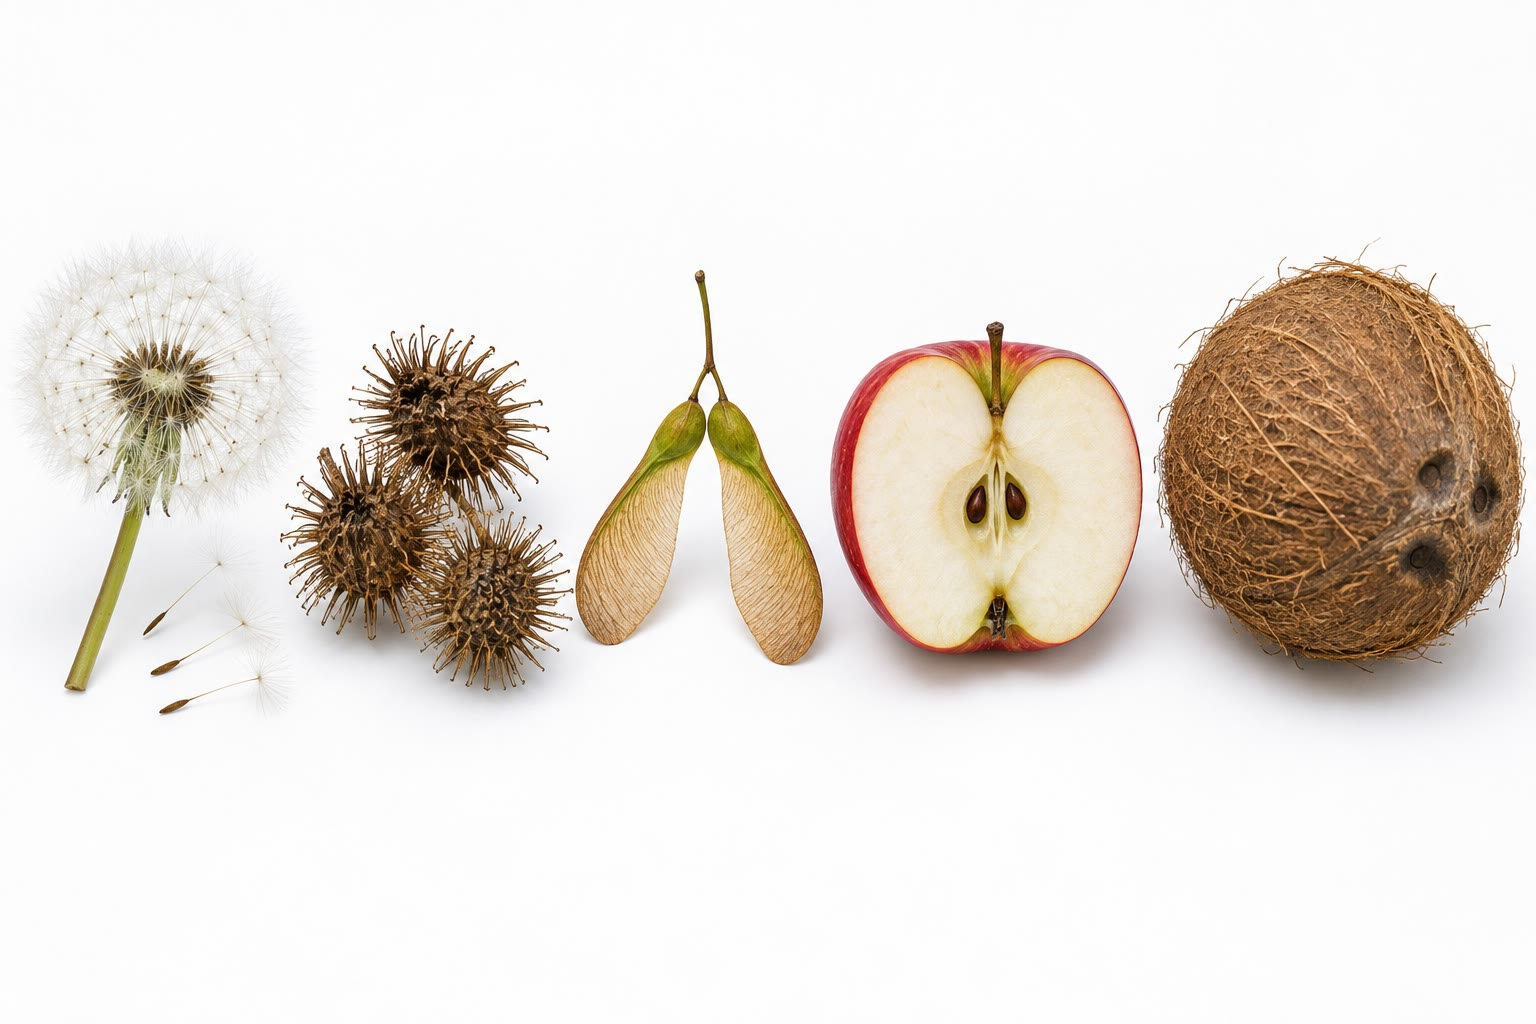
\includegraphics[width=0.62\linewidth]{images/book4/ai/b4-06-fruits-seeds.jpg}

{\small \omterm{def:b2:angiosperm-reproduction:seed}{Frutos} feitos para a dispersão: paraquedas (dente-de-leão),
ganchos (bardana), asas (bordo), polpa para um animal (maçã) e uma
casca flutuante para o mar (coco).}
\end{omfigure}

\begin{example}[Distâncias de dispersão]\label{ex:b2:angiosperm-reproduction:dispersal}
Um aquênio de dente-de-leão com seu paraquedas desce a
\qty{0.3}{m/s}; a partir de \qty{0.3}{m}, num vento de \qty{3}{m/s},
ele voa \qty{3}{m} e, numa corrente térmica, centenas. Uma sâmara de
bordo desce em autorrotação a \qty{1}{m/s} a partir de \qty{15}{m}:
\qty{45}{m}. Um caroço de cereja largado por uma ave depois de um voo
de vinte minutos a \qty{10}{m/s}: até \qty{12}{km}. As bolotas de um
carvalho caem a seus pés, a menos que um gaio as leve, o que ele faz
aos milhares, a um quilômetro ou mais, esquecendo um décimo delas: os
carvalhos que recolonizaram a Europa depois da última glaciação
avançaram para o norte a centenas de metros por ano, muito mais
depressa do que uma bolota rola, e foram as aves que os levaram.
\end{example}

\section{Exercícios}

\begin{exercise}[$\star$]\label{exo:b2:angiosperm-reproduction:1}
Cite os quatro verticilos de uma \omterm{def:b2:angiosperm-reproduction:flower}{flor} e as partes de um \omterm{def:b2:angiosperm-reproduction:flower}{estame} e de um
\omterm{def:b2:angiosperm-reproduction:flower}{carpelo}. Quais partes são \omterm{def:b2:plant-life-cycles:cycles}{esporófito} \omterm{def:b2:meiosis-heredity:meiosis}{diploide}, e quais são \omterm{def:b2:plant-life-cycles:cycles}{gametófito}
\omterm{def:b2:meiosis-heredity:meiosis}{haploide}?
\end{exercise}

\begin{exercise}[$\star$]\label{exo:b2:angiosperm-reproduction:2}
Dê a ploidia de: um \omterm{def:b2:plant-life-cycles:heterospory}{micrósporo}, a célula vegetativa, uma célula
espermática, a oosfera, um núcleo polar, o zigoto, o endosperma, o
\omterm{def:b2:angiosperm-reproduction:seed}{tegumento da semente}, a parede do \omterm{def:b2:angiosperm-reproduction:seed}{fruto}.
\end{exercise}

\begin{exercise}[$\star$]\label{exo:b2:angiosperm-reproduction:3}
Liste cinco traços de uma \omterm{def:b2:angiosperm-reproduction:flower}{flor} polinizada pelo vento e cinco de uma
\omterm{def:b2:angiosperm-reproduction:flower}{flor} polinizada por abelhas, e dê uma planta para cada uma.
\end{exercise}

\begin{exercise}[$\star$]\label{exo:b2:angiosperm-reproduction:4}
O que é a \omterm{prop:b2:angiosperm-reproduction:double}{dupla fecundação}, e o que é produzido por cada uma das duas
fusões? Por que se pode dizer que o endosperma é ``feito sob
encomenda''?
\end{exercise}

\begin{exercise}[$\star\star$]\label{exo:b2:angiosperm-reproduction:5}
Um cabelo de milho tem \qty{25}{cm} de comprimento, e um \omterm{thm:b2:angiosperm-reproduction:tube}{tubo polínico}
cresce a \qty{1.2}{cm/h}. Quanto tempo a fecundação leva após a
\omterm{def:b2:angiosperm-reproduction:pollination}{polinização}? Um pendão libera \omterm{def:b2:plant-life-cycles:heterospory}{pólen} do dia 0 ao dia 7, e os cabelos da
planta emergem do dia 5 ao dia 12, um oitavo deles a cada dia; um
cabelo só capta \omterm{def:b2:plant-life-cycles:heterospory}{pólen} enquanto houver liberação de \omterm{def:b2:plant-life-cycles:heterospory}{pólen}. Que fração
dos cabelos é polinizada?
\end{exercise}

\begin{exercise}[$\star\star$]\label{exo:b2:angiosperm-reproduction:6}
Sob autoincompatibilidade gametofítica, que fração do \omterm{def:b2:plant-life-cycles:heterospory}{pólen} é
compatível nos cruzamentos $S_1S_2\times S_1S_2$, $S_1S_2\times
S_1S_3$, $S_1S_2\times S_3S_4$ (o pistilo indicado primeiro)? Dê os
\omterm{def:b2:meiosis-heredity:vocabulary}{genótipos} dos descendentes do segundo cruzamento.
\end{exercise}

\begin{exercise}[$\star\star$]\label{exo:b2:angiosperm-reproduction:7}
Numa população com $n$ \omterm{def:b2:meiosis-heredity:vocabulary}{alelos} $S$ igualmente frequentes, que fração do
\omterm{def:b2:plant-life-cycles:heterospory}{pólen} tomado ao acaso é compatível com uma dada planta? Explique por
que um novo \omterm{def:b2:meiosis-heredity:vocabulary}{alelo} $S$ surgido por \omterm{def:b2:genome-diversification:mutation}{mutação} se espalha, e o que isso
prevê para o número de \omterm{def:b2:meiosis-heredity:vocabulary}{alelos}.
\end{exercise}

\begin{exercise}[$\star\star$]\label{exo:b2:angiosperm-reproduction:8}
Uma planta de milho heterozigota $Yy$ (endosperma amarelo \omterm{def:b2:meiosis-heredity:vocabulary}{dominante}) é
autofecundada. Dê os \omterm{def:b2:meiosis-heredity:vocabulary}{genótipos} do endosperma de seus grãos e suas
proporções, lembrando que os dois \omterm{prop:b2:angiosperm-reproduction:embryosac}{núcleos polares} são idênticos. Que
fração dos grãos é amarela? E se a planta for polinizada por uma planta
$yy$?
\end{exercise}

\begin{exercise}[$\star\star$]\label{exo:b2:angiosperm-reproduction:9}
Descreva o experimento da aleurona e explique o que ele mostra sobre
(a) o papel do embrião, (b) o papel da giberelina, (c) o local de
síntese da amilase. Por que uma metade de grão sem embrião é o controle
essencial?
\end{exercise}

\begin{exercise}[$\star\star\star$]\label{exo:b2:angiosperm-reproduction:10}
Compare o custo das estratégias do vento e dos animais: uma planta
polinizada pelo vento produz $10^{6}$ grãos por \omterm{def:b2:plant-life-cycles:heterospory}{óvulo}, a
\qty{1}{\micro g} cada; uma planta polinizada por animais produz
$10^{3}$ grãos por \omterm{def:b2:plant-life-cycles:heterospory}{óvulo}, a \qty{1}{\micro g} cada, mais \qty{5}{mg}
de açúcar de \omterm{def:b2:angiosperm-reproduction:pollination}{néctar} por \omterm{def:b2:angiosperm-reproduction:flower}{flor} de dez \omterm{def:b2:plant-life-cycles:heterospory}{óvulos}. Calcule o custo reprodutivo
por \omterm{def:b2:plant-life-cycles:heterospory}{óvulo} em cada caso (considere \omterm{def:b2:plant-life-cycles:heterospory}{pólen} e açúcar com a mesma energia
por grama), e explique por que a \omterm{def:b2:angiosperm-reproduction:pollination}{polinização} pelo vento persiste mesmo
assim.
\end{exercise}

\begin{exercise}[$\star\star\star$]\label{exo:b2:angiosperm-reproduction:11}
Explique, com os números do \cref{ex:b2:angiosperm-reproduction:dispersal},
por que um \omterm{def:b2:angiosperm-reproduction:seed}{fruto} carnoso vale seu custo para uma árvore, embora o
animal digira a polpa e deixe cair a maioria das \omterm{def:b2:angiosperm-reproduction:seed}{sementes} onde elas não
podem crescer.
\end{exercise}

\begin{exercise}[$\star\star\star$]\label{exo:b2:angiosperm-reproduction:12}
``O \omterm{def:b2:angiosperm-reproduction:flower}{carpelo} fechado é a razão pela qual as plantas com \omterm{def:b2:angiosperm-reproduction:flower}{flores} dominam
a terra firme.'' Discuta: o que o encerramento do \omterm{def:b2:plant-life-cycles:heterospory}{óvulo} torna possível
(escolha do \omterm{def:b2:plant-life-cycles:heterospory}{pólen}, incompatibilidade, o \omterm{def:b2:angiosperm-reproduction:seed}{fruto}) e o que ele custa.
\end{exercise}

\section{Problema: Um pomar e uma lavoura}

\begin{problem}[{Problema de fim de semana --- a polinização de um pomar
de macieiras planejada em torno da autoincompatibilidade, e a
fecundação e a produtividade de uma lavoura de milho calculadas a
partir do pólen que ela produz, até a frutificação do pomar e o número
de grãos da lavoura}]
\label{pb:b2:angiosperm-reproduction:1}
A macieira é gametofiticamente autoincompatível. Um pomar tem três
variedades: A ($S_1S_2$), B ($S_1S_3$), C ($S_3S_4$). Uma \omterm{def:b2:angiosperm-reproduction:flower}{flor} tem cinco
\omterm{def:b2:angiosperm-reproduction:flower}{carpelos} com dois \omterm{def:b2:plant-life-cycles:heterospory}{óvulos} cada, e um \omterm{def:b2:angiosperm-reproduction:seed}{fruto} que forma menos de cinco
\omterm{def:b2:angiosperm-reproduction:seed}{sementes} é descartado pela árvore. Uma visita de abelha deposita
\num{100} \omterm{prop:b2:angiosperm-reproduction:pollen}{grãos de pólen} num \omterm{def:b2:angiosperm-reproduction:flower}{estigma}; cada grão compatível tem
probabilidade $0.1$ de fecundar um \omterm{def:b2:plant-life-cycles:heterospory}{óvulo} ainda não ocupado. Uma árvore
tem \num{5000} \omterm{def:b2:angiosperm-reproduction:flower}{flores} e precisa de \num{250} \omterm{def:b2:angiosperm-reproduction:seed}{frutos} para uma safra
completa. Milho: um pendão libera $10^{7}$ grãos ao longo de \num{7}
dias; a lavoura tem \num{8} plantas por metro quadrado; uma planta tem
uma espiga de \num{600} cabelos; um cabelo apresenta
\qty{1e-4}{m^2} ao \omterm{def:b2:plant-life-cycles:heterospory}{pólen} que cai; o \omterm{def:b2:plant-life-cycles:heterospory}{pólen} sedimenta a
\qty{0.25}{m/s}; um grão de milho contém \qty{0.3}{g} de endosperma.

\medskip
\noindent\textbf{Parte I --- Compatibilidade.}
\begin{enumerate}
  \item Para o \omterm{def:b2:plant-life-cycles:heterospory}{pólen} de cada variedade sobre um pistilo de A, dê a
        fração compatível $f$.
  \item O mesmo para pistilos de B e de C.
  \item Uma abelha que chega de uma árvore de B deposita 100 grãos
        num \omterm{def:b2:angiosperm-reproduction:flower}{estigma} de A: quantos são compatíveis, e quantos \omterm{def:b2:plant-life-cycles:heterospory}{óvulos} se
        espera que sejam fecundados (despreze a saturação)?
  \item O mesmo para uma abelha vinda de C, e de outra A.
  \item Quais \omterm{def:b2:angiosperm-reproduction:seed}{frutos} são mantidos? Qual é o risco de plantar um pomar
        só da variedade A?
  \item Um bloco de árvores A é cercado por árvores C; metade das
        visitas de abelhas às A vem de C. Se cada \omterm{def:b2:angiosperm-reproduction:flower}{flor} recebe uma
        visita, que fração das \omterm{def:b2:angiosperm-reproduction:flower}{flores} de A frutifica, e quantos \omterm{def:b2:angiosperm-reproduction:seed}{frutos}
        há por árvore? A safra é completa?
  \item Por que os pomares intercalam uma macieira silvestre que
        floresce durante semanas, e por que é preciso verificar seus
        \omterm{def:b2:meiosis-heredity:vocabulary}{alelos} $S$?
\end{enumerate}

\medskip
\noindent\textbf{Parte II --- O \omterm{def:b2:plant-life-cycles:heterospory}{pólen} sobre a lavoura de milho.}
\begin{enumerate}[resume]
  \item Calcule o \omterm{def:b2:plant-life-cycles:heterospory}{pólen} liberado por metro quadrado de lavoura por
        segundo, em média ao longo dos sete dias.
  \item Em regime estacionário, o fluxo de \omterm{def:b2:plant-life-cycles:heterospory}{pólen} que sedimenta é igual
        à taxa de liberação. Calcule a concentração de \omterm{def:b2:plant-life-cycles:heterospory}{pólen} no ar
        (grãos por metro cúbico).
  \item Calcule o número de grãos que caem sobre um cabelo por segundo
        e o tempo médio de espera pelo primeiro grão.
  \item Quantos grãos um cabelo recebe num dia? Por que só o primeiro é
        útil?
  \item Um cabelo de \qty{20}{cm} é polinizado; o tubo cresce a
        \qty{1}{cm/h}. Quando o \omterm{def:b2:plant-life-cycles:heterospory}{óvulo} é fecundado?
  \item Uma seca atrasa em cinco dias a emergência dos cabelos,
        enquanto o pendão libera \omterm{def:b2:plant-life-cycles:heterospory}{pólen} no prazo normal. Usando o período
        de liberação de sete dias, estime a fração da estação de \omterm{def:b2:plant-life-cycles:heterospory}{pólen}
        que os cabelos aproveitam, e a consequência para a
        produtividade.
\end{enumerate}

\medskip
\noindent\textbf{Parte III --- A \omterm{prop:b2:angiosperm-reproduction:double}{dupla fecundação} e o grão.}
A lavoura é de uma variedade de endosperma amarelo ($Y$, \omterm{def:b2:meiosis-heredity:vocabulary}{dominante}),
vizinha de uma lavoura branca ($yy$); o vento sopra da lavoura branca.
\begin{enumerate}[resume]
  \item Dê os \omterm{def:b2:meiosis-heredity:vocabulary}{genótipos} do embrião e do endosperma de um grão de uma
        planta $YY$ fecundada por \omterm{def:b2:plant-life-cycles:heterospory}{pólen} $yy$.
  \item O grão é amarelo ou branco? Explique o termo xênia.
  \item Uma planta $Yy$ é polinizada por \omterm{def:b2:plant-life-cycles:heterospory}{pólen} $yy$: dê os \omterm{def:b2:meiosis-heredity:vocabulary}{genótipos} do
        endosperma e suas frequências.
  \item O endosperma contém dois genomas maternos e um paterno. Um gene
        com efeito de dose dá, por cópia, 10~unidades de pigmento: que
        quantidade de pigmento têm os grãos $YYy$, $Yyy$ e $yyY$ (duas
        doses paternas, por hipótese)? Quais deles podem de fato
        existir?
  \item Explique por que o que comemos é o endosperma, e não o
        embrião, e que fração da massa do grão ele representa se o
        embrião pesa \qty{0.03}{g}.
  \item Por que o abastecimento ``sob encomenda'' do endosperma é uma
        vantagem sobre o das gimnospermas?
\end{enumerate}

\medskip
\noindent\textbf{Parte IV --- Produtividade.}
\begin{enumerate}[resume]
  \item Se \qty{90}{\%} dos cabelos forem fecundados, calcule os grãos
        por espiga, por planta e por metro quadrado, e a massa de
        endosperma por metro quadrado.
  \item Converta em toneladas por hectare.
  \item A lavoura fixa \qty{1.2}{kg} de carbono por metro quadrado por
        estação, dos quais metade termina no grão colhido. Verifique a
        coerência com a massa da questão 20 (o endosperma tem
        \qty{45}{\%} de carbono).
  \item Quantos \omterm{prop:b2:angiosperm-reproduction:pollen}{grãos de pólen} a lavoura liberou por grão colhido?
  \item Explique por que um pé de milho isolado numa horta forma uma
        espiga mal granada.
  \item Enuncie o resultado: a frutificação do bloco A e a
        produtividade da lavoura em grãos por metro quadrado e em
        toneladas por hectare.
\end{enumerate}
\end{problem}
